\documentclass[pdflatex,compress]{beamer}

%\usetheme[dark,framenumber,totalframenumber]{ElektroITK}
\usetheme[darktitle,framenumber,totalframenumber]{ElektroITK}
\usepackage{graphicx}
\usepackage{multicol}

\title{Data Communications}
\subtitle{Chapter 4 - Transmission Media}

\author{Mifta Nur Farid}

\begin{document}

\maketitle

\begin{frame}
	\frametitle{Design Factors Determining Data Rate and Distance}
	\begin{itemize}
		\item \textbf{Bandwidth}\\
		Higher bandwidth gives higher data rate
		\item \textbf{Transmission impairments}\\
		Impairments, such as attenuation, limit the distance
		\item \textbf{Interference}\\
		Overlapping frequency bands can distort or wipe out a signal
		\item \textbf{Number of receivers}\\
		More receivers introduces more attenuation
	\end{itemize}
\end{frame}

\begin{frame}
	\begin{center}
		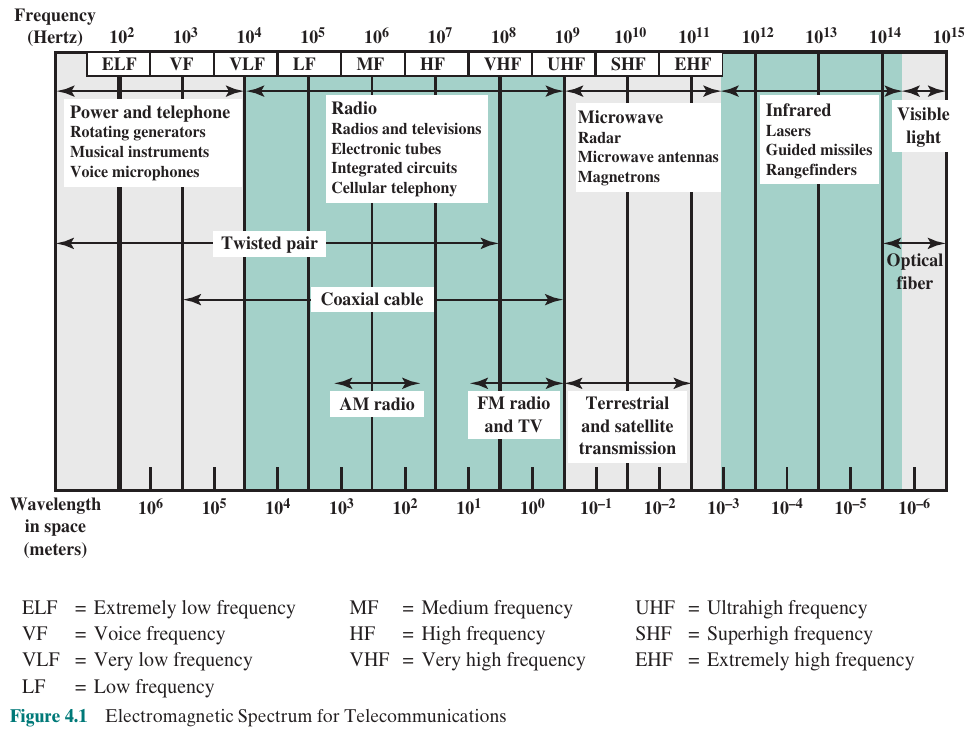
\includegraphics[width=0.9\linewidth]{img/img01}
	\end{center}
\end{frame}

\begin{frame}
	\begin{center}
		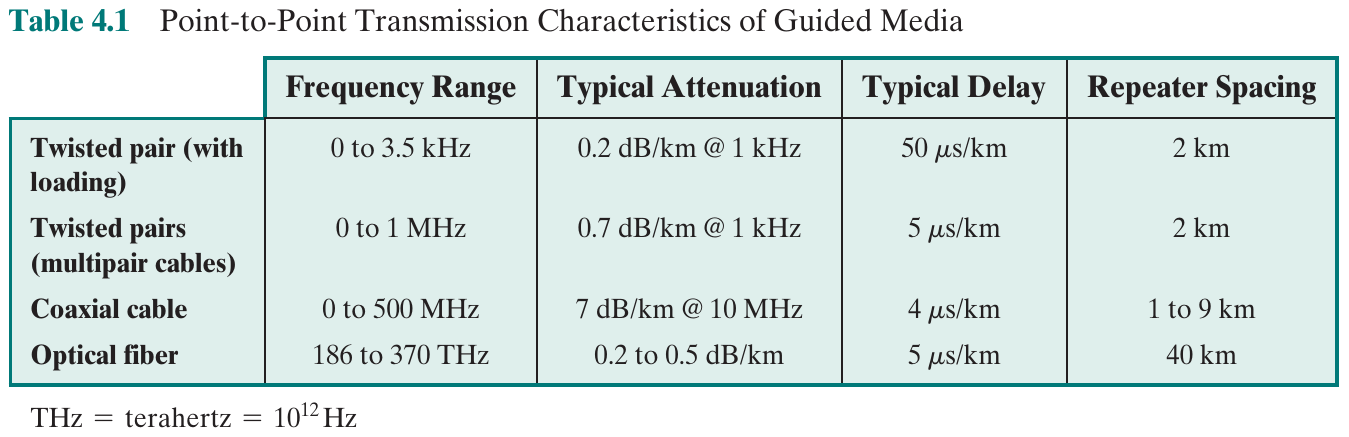
\includegraphics[width=\linewidth]{img/img02}
	\end{center}
\end{frame}

\begin{frame}
	\begin{center}
		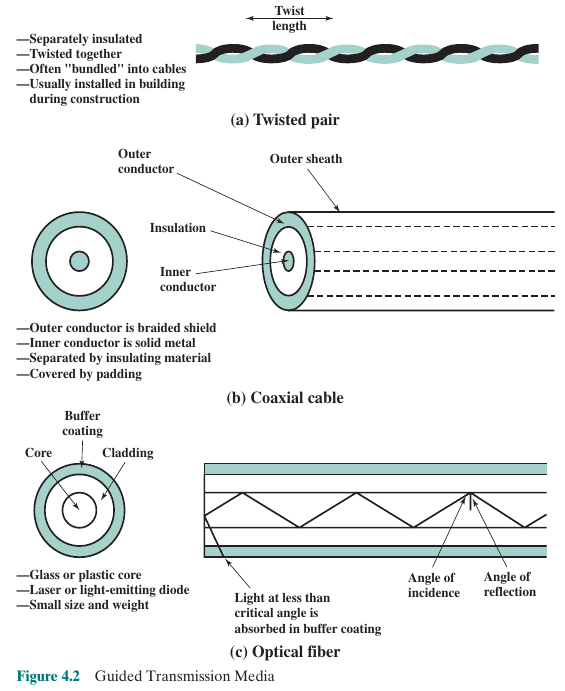
\includegraphics[width=0.5\linewidth]{img/img03a}
	\end{center}
\end{frame}

\begin{frame}
	\frametitle{Twisted Pair}
	\begin{itemize}
		\item Twisted pair is the least expensive and most widely used guided transmission medium
		\begin{center}
			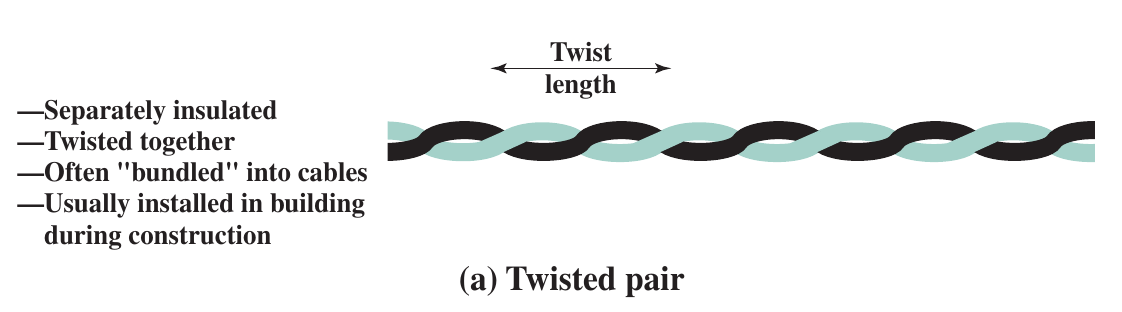
\includegraphics[width=0.8\linewidth]{img/img03}
		\end{center}
		\item Consists of two insulated copper wires arranged in a regular spiral pattern
		\item A wire pair acts as a single communication link
		\item Pairs are bundled together into a cable
		\item Most commonly used in the telephone network and for communications within buildings
	\end{itemize}
\end{frame}

\begin{frame}
	\begin{center}
		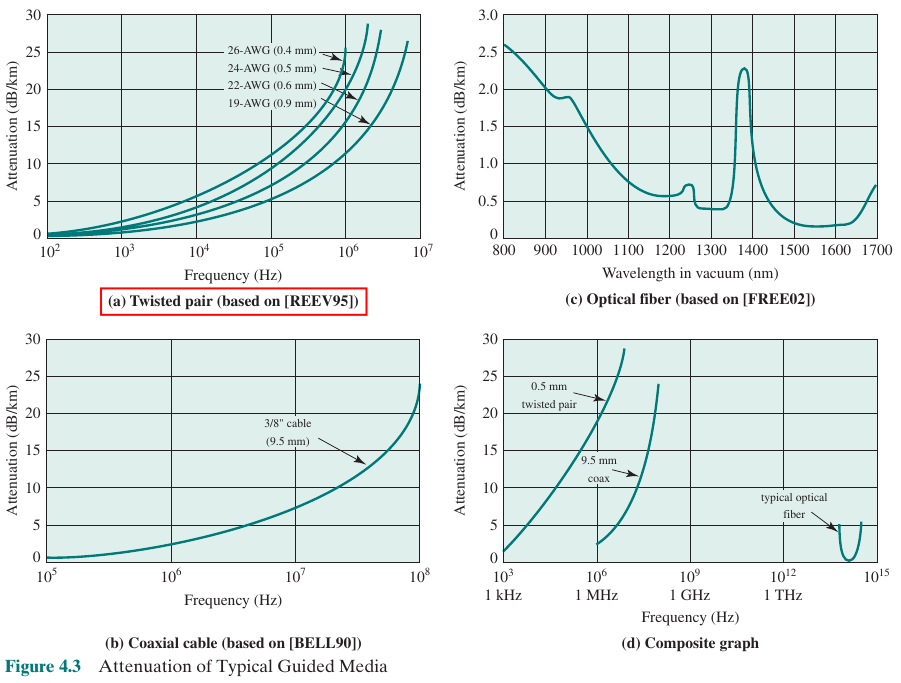
\includegraphics[width=0.8\linewidth]{img/img06}
	\end{center}
\end{frame}

\begin{frame}
	\frametitle{Unshielded and Shielded Twisted Pair}
	\begin{enumerate}
		\item Unshielded Twisted Pair (UTP)
		\begin{itemize}
			\item  Consists of one or more twisted-pair cables, typically enclosed within an overall thermoplastic jacket which provides no electromagnetic shielding
			\item Ordinary telephone wire
			\item Subject to external electromagnetic interference
			\item The tighter the twisting, the higher the supported transmission rate and the greater the cost per meter
		\end{itemize}
		\item Shielded Twisted Pair (STP)
		\begin{itemize}
			\item Has metal braid or sheathing that reduces interference
			\item Provides better performance at higher data rates
			\item More expensive
		\end{itemize}
	\end{enumerate}	
\end{frame}

\begin{frame}
	\begin{center}
		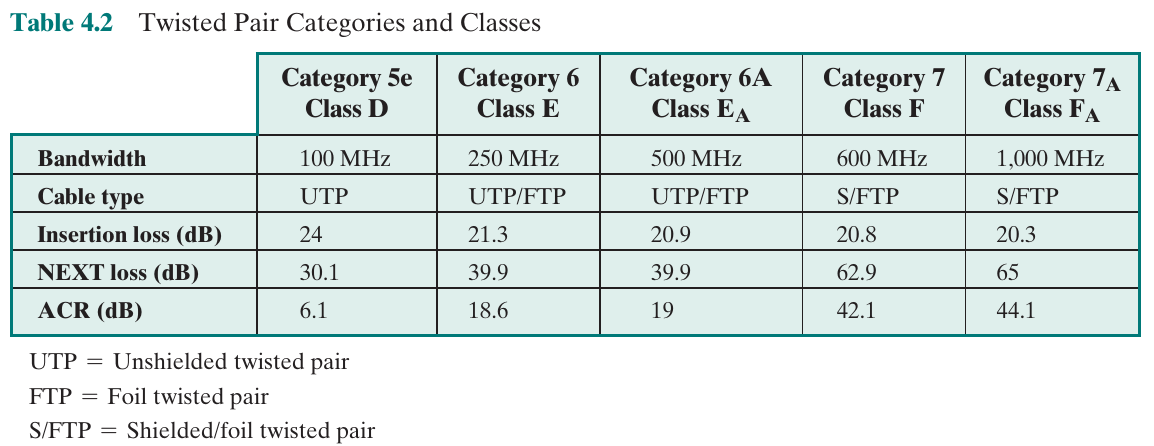
\includegraphics[width=\linewidth]{img/img07}
	\end{center}
\end{frame}

\begin{frame}
	\frametitle{Twisted Pair}
	\begin{center}
		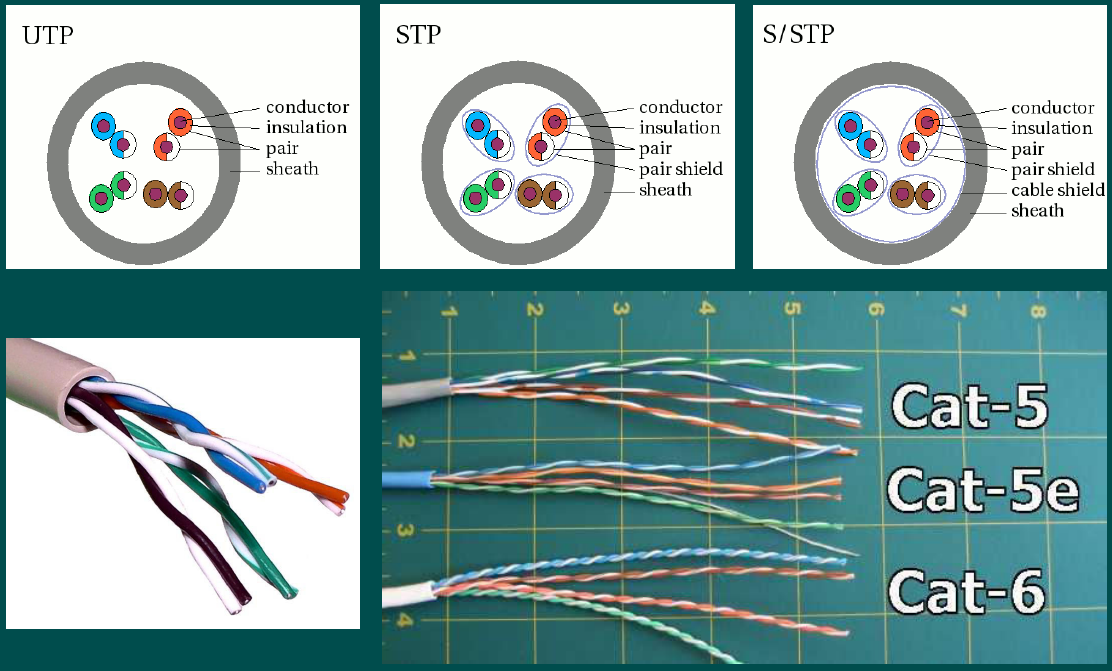
\includegraphics[width=\linewidth]{img/img08}
	\end{center}
\end{frame}

\begin{frame}
	\frametitle{Near-End Crosstalk (NEXT)}
	\begin{itemize}
		\item Coupling of signal from one pair of
		conductors to another
		\begin{itemize}
			\item Conductors may be the metal pins in a connector or wire pairs in a cable
		\end{itemize}
		\item Near end refers to coupling that takes place when the transmit signal entering the link couples back to the receive conductor pair at that same end of the link
		\item Greater NEXT loss magnitudes are associated with less crosstalk noise
	\end{itemize}
\end{frame}

\begin{frame}
	\begin{center}
		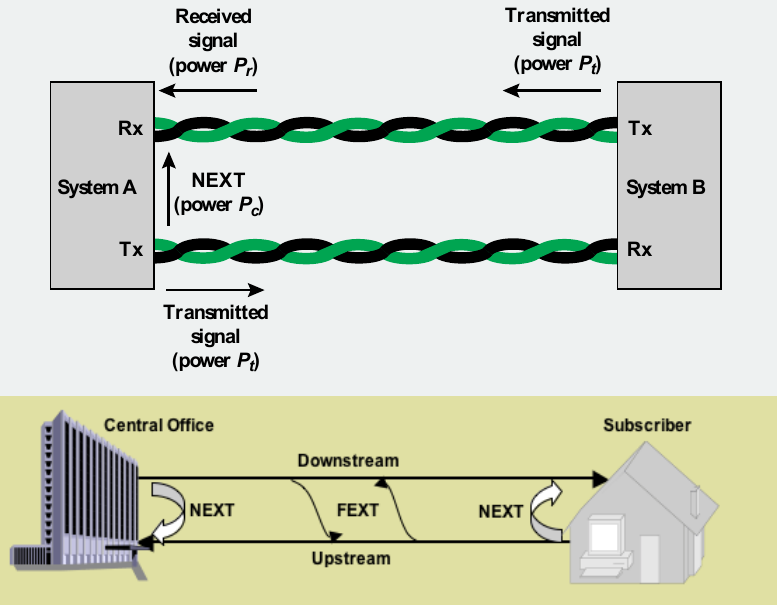
\includegraphics[width=0.8\linewidth]{img/img09}
	\end{center}
\end{frame}

\begin{frame}
	\begin{center}
		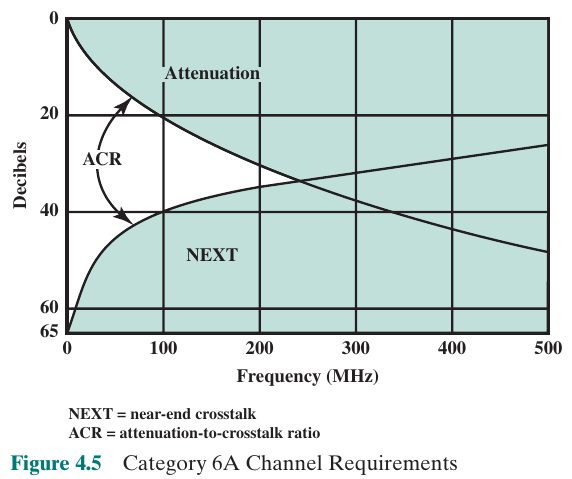
\includegraphics[width=0.7\linewidth]{img/img10}
	\end{center}
\end{frame}

\begin{frame}
	\frametitle{Coaxial Cabel}
	\begin{itemize}
		\item Coaxial cable can be used over longer distances and support more stations on a shared line than twisted pair
		\begin{center}
			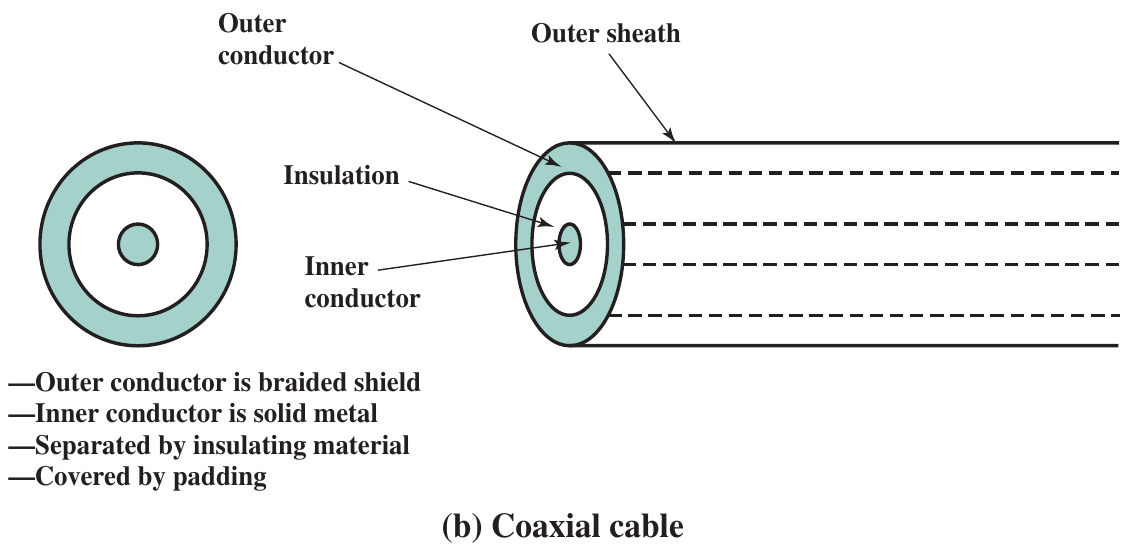
\includegraphics[width=0.5\linewidth]{img/img04}
		\end{center}
		\item Consists of a hollow outer cylindrical conductor that surrounds a single inner wire conductor
		\item Is a versatile transmission medium used in a wide variety of applications
		\item Used for TV distribution, long distance telephone transmission and LANs
	\end{itemize}
\end{frame}

\begin{frame}
	\frametitle{Coaxial Cable - Transmission Characteristics}
	\begin{itemize}
		\item Frequency characteristics superior to twisted pair
		\item Performance limited by attenuation and noise
		\item Analog signals
		\begin{itemize}
			\item  Amplifiers are needed every few kilometers - closer if higher frequency
			\item Usable spectrum extends up to 500MHz
		\end{itemize}
		\item Digital signals
		\begin{itemize}
			\item Repeater every 1 km - closer for higher data rates
		\end{itemize}
	\end{itemize}
	\begin{center}
		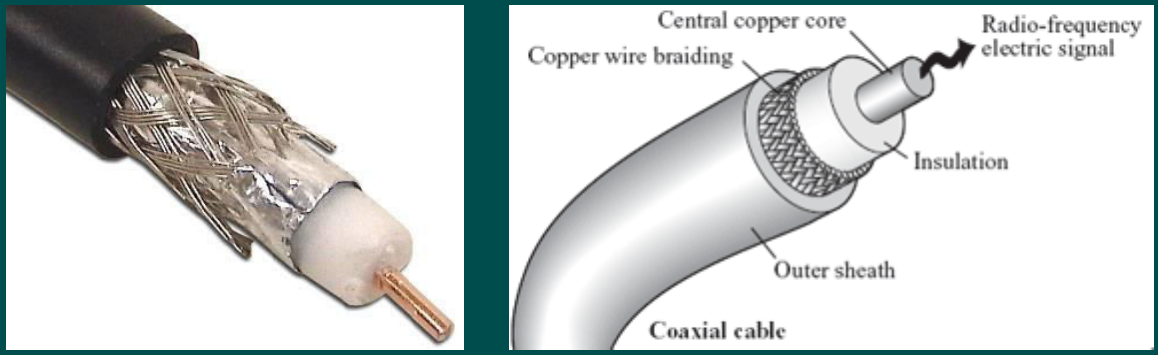
\includegraphics[width=0.7\linewidth]{img/img11}
	\end{center}
\end{frame}

\begin{frame}
	\begin{center}
		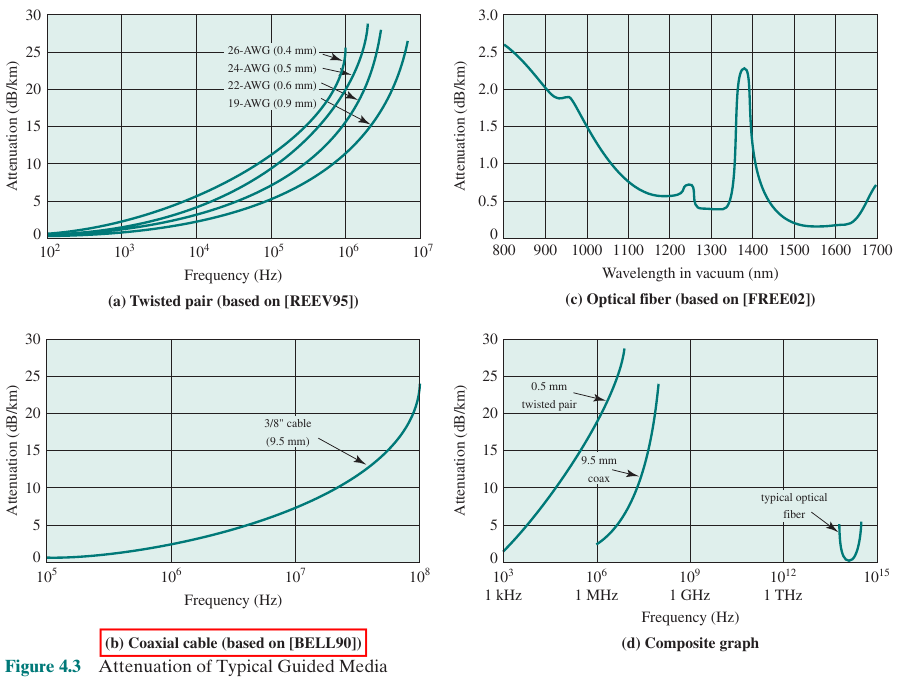
\includegraphics[width=0.8\linewidth]{img/img12}
	\end{center}
\end{frame}

\begin{frame}
	\frametitle{Optical Fiber}
	\begin{itemize}
		\item Optical fiber is a thin flexible medium capable of guiding an optical ray
		\begin{center}
			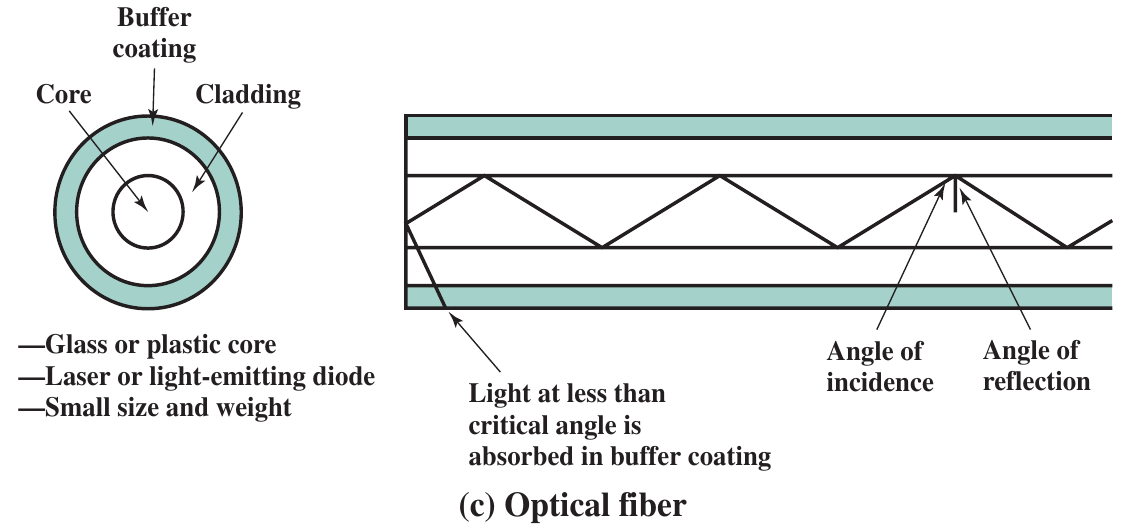
\includegraphics[width=0.5\linewidth]{img/img05}
		\end{center}
		\item Various glasses and plastics can be used to make optical fibers
		\item Has a cylindrical shape with three sections – core, cladding, jacket
		\item Widely used in long distance telecommunications
		\item Performance, price and advantages have made it popular to use
	\end{itemize}
\end{frame}

\begin{frame}{Optical Fiber}
	\begin{center}
		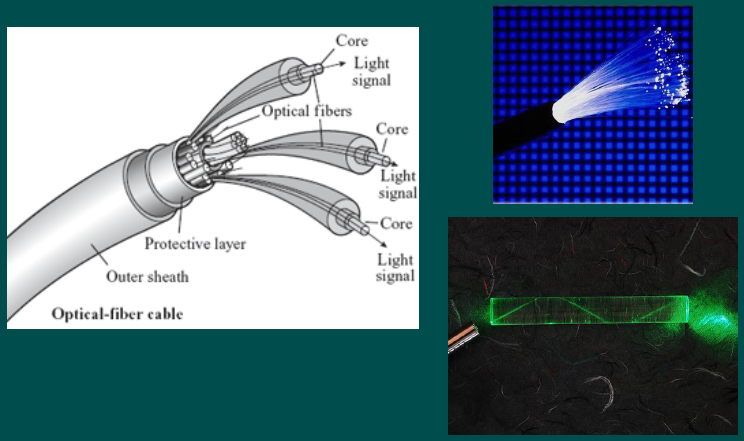
\includegraphics[width=\linewidth]{img/img13}
	\end{center}
\end{frame}

\begin{frame}
	\frametitle{Tugas Mandiri}
	\begin{itemize}
		\item Stallings, W. (2014). Data and Computer Communications, 10th Edition, New Jersey: Upper Saddle River\\
		\begin{itemize}
			\item Chapter 2 Protocol Architecture, TCP/IP, and Internet-Based Applications
		\end{itemize}
		\item Gupta, P. C. (2006). Data Communications and Computer Networks. New Delhi: Prentice Hall of India\\
		\begin{itemize}
			\item Section 6.8 Layered Architecture of the OSI Reference Model.
			\item Section 6.14.1 TCP/IP
		\end{itemize}
		\item Tanenbaum, A. S. \& Wetherall, D. J. (2013). Computer Networks, Fifth Edition. London: Pearson.\\
		\begin{itemize}
			\item Section 3.1 Protocol Hierarchies
		\end{itemize}
	\end{itemize}
\end{frame}

\begin{frame}
	\frametitle{Tugas Terstruktur}
	\textbf{Tampilkan Tugas 2}
\end{frame}

\end{document}
